%---------------------------------------------------------------------------
% System tests.
%
%---------------------------------------------------------------------------
\section{System Tests}
\label{sec:tests}
\subsection{Performance tests}

In order to evaluate system performance abilities and to find potential bottlenecks, load tests were performed. Due to lack of resources, setup used for this purpose was rather simple. For test purposes I have used 2 machines: 

\begin{itemize}
\item {\bf HP nx6110} laptop having Pentium M 1.73 GHz CPU and 1.5GB of RAM, running Ubuntu Linux
\item {\bf Sony Vaio VPCEB2Z1E}, with Pentium i5 M430, running at 2.24GHz with 2 physical cores and two processing pipelines running on each core, additionally having 4GB of RAM. This machine was running Microsoft Windows7.
\end{itemize}
Those machines where connected using 100Mb Fast Ethernet switch.
Test scenario was composed of following steps:
\begin{enumerate}
\item Launch Monitoring Hub Application module
\item Launch GUI module
\item On separate machine launch 3 JVM processes that mimic processing workflow
\item Again, on testing machine launch iptraf to have insight to network load
\item Launch 2 JProfiler\footnote{\url{http://www.ej-technologies.com/products/jprofiler/overview.html}} instances, attach them to GUI and Monitoring Hub processes
\item Using GUI module and external Monitoring Hub Application started in previous step, add all 3 JVMs as measured resources
\item Create 20 sample measurements, covering: Memory usage, CPU usage, per process Heap and Non Heap memory usage
\item Create 5 Visualizations, using all types that system supports and measurements created in previous step
\item Let the system running for a while, so it is possible to gather performance data of system being on severe load
\item Dispose visualizations
\item Dispose measurements
\item Remove resources
\item Leave system running for short period of time, to make sure that CPU and memory usage returns to values from idle state
\end{enumerate}

In designed scenario, I am using external Monitoring Hub Application to verify resources usage of each component separately. Additionally, HP laptop was running test application and Vaio was running monitoring system. I have decided to use those resources in that way, to make sure that system being tested will not reach machine limits to be certain that results aren\rq{}t polluted with edge conditions. Results of tests can be found below.

\begin{figure}[ht]
\centering
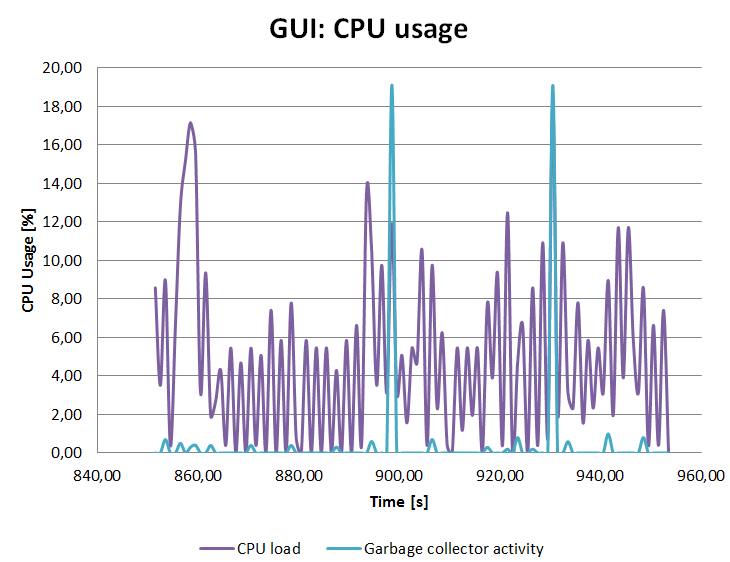
\includegraphics[width=0.6\textwidth]{prof_GUI_CPU}
\caption{Profiling results of GUI component - CPU usage perspective}
\label{fig:prof_GUI_CPU}
\end{figure}

Figures~\ref{fig:prof_GUI_CPU}~and~\ref{prof_GUI_MEM}~depicts JVM telemetry measurements produced by JProfiler during stage of tests where system where operating under heaviest load (Step~9 from list above). As can be seen, system never consumed more than 90MB of used memory. The maximum of commit memory slightly exceeded 140MB. On the other hand, the CPU time spent on actual data processing never reached 18\%, having an average between 2\% and 8\%. What is quite interesting is the Garbage Collection, most of the time CPU time spent on garbage collection was hardly traceable, but there were 2 peaks where GC consumed nearly 20\% of CPU time. 

\begin{figure}[ht]
\centering
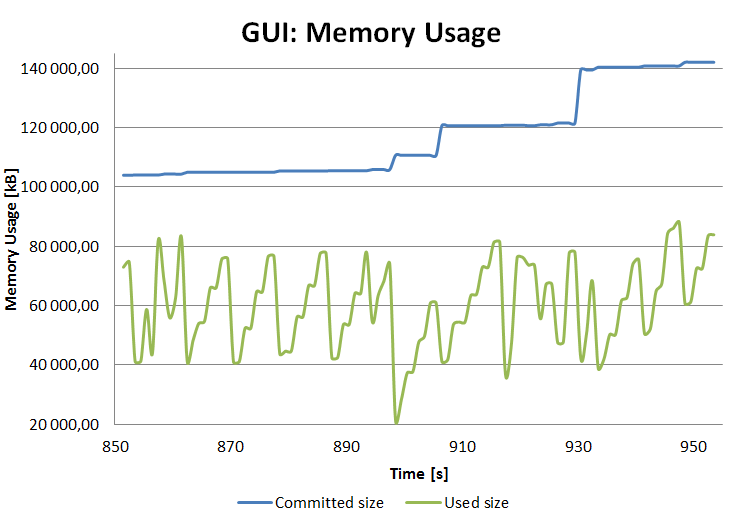
\includegraphics[width=0.6\textwidth]{prof_GUI_MEM}
\caption{Profiling results of GUI component - memory usage perspective}
\label{fig:prof_GUI_MEM}
\end{figure}
\begin{figure}[ht]
\centering
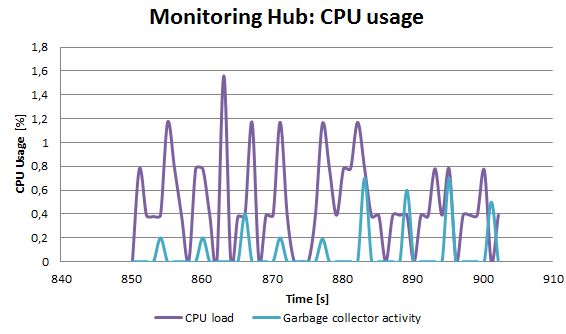
\includegraphics[width=0.6\textwidth]{prof_mon_hub_CPU}
\caption{Profiling results of Monitoring Hub component - CPU usage perspective}
\label{fig:prof_mon_hub_CPU}
\end{figure}

As it is easily predictable, the Monitoring Hub module was consuming significantly smaller portion of resources then the GUI. Figures~\ref{fig:prof_mon_hub_CPU}~and~\ref{fig:prof_mon_hub_mem} covers telemetry of Monitoring Hub JVM process in same time frame (step 9 of test scenario). Module\rq{}s CPU usage was only fraction of GUI usage - peak was about 1.6\%. Regarding memory usage - Those values also were smaller than in GUI but significant - memory really used by application was staying in 10-20MB range, commit memory was nearly constant and equal to approximately 50MB.

Additionally network usage rendered by iptraf showed near constant bit rate equal to 130kbps.
\begin{figure}[ht]
\centering
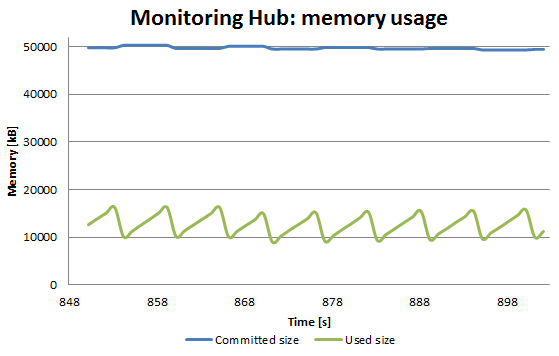
\includegraphics[width=0.6\textwidth]{prof_mon_hub_mem}
\caption{Profiling results of Monitoring Hub component - memory usage perspective}
\label{fig:prof_mon_hub_mem}
\end{figure}

Test results showed clearly that performance of proposed system is good enough to say that there aren\rq{}t any significant bottlenecks. Additionally, really low resources usage of Monitoring Hub builds solid scaffold for further scaling the application up.

Such a good results could be obtained mostly by keeping code that is responsible for processing measurements really simple and optimized. Measurement processing consists only of gathering data and transmitting them to other layers.

\subsection{Usability tests}

As was previously stated, in the beginning of this chapter, in order to prove that system is really useful, test with real world application were performed. In this subsection, I will cover this test - from stating the problem, describing solution, implemented test application ending up with benefits that SemSimMon gives application author.

Let us assume that we\rq{}ve got an assignment - create an application that will solve linear problems and that will provide basic Web UI for accessing its services. Application should allow user to provide any square linear system using UI and will render result vector in same view. Application should optimize response time rather than high throughput. Additionally, to ensure response time, proposed solution shall operate on MPI-powered cluster and external server machine that is capable of running HTTP server application. Both cluster and HTTP server machine have same NFS share attached. 

Solution to above problem is a system consisting two modules: web application providing interface and processing application that solves the equations and runs on MPI cluster. Web application submits jobs for the cluster using NFS share, by creating request file. Solving module, checks for new jobs by polling for new request file, solves the equation and then generates response file. Web application, after submitting new job file, simply waits for solution by polling same NFS share for result file. 

System was implemented as a J2EE application and standalone, parallel application for solving equations. Sources of both components can be found in test-webapp module along with rest of SemSimMon components.

After implementing above application, one should try to analyze its behavior under some load. Due to same lack of resources, tests were performed on cluster, composed of 2 virtual nodes. Virtual nodes were created using Oracle VirtualBox platform, and both were running 32-bit Ubuntu 9.10. The first, main node was running both HTTP server and main node of equations solving cluster. The second node was just computing one.

For measuring load purposes, I have been using SemSimMon running on Guest (Windows 7) OS. After attaching to all resources, I have started measuring basic capabilities - CPU Time, memory usage and general system load. As it was expected, CPU usage of HTTP server was minimal (approx. 1-5\%), although it could be smaller. The measured usage is mostly due to polling for result file. The memory usage is almost constant - non-heap area was definitely constant, approximately 24.MB. The heap memory was varying between 4MB - 7MB.

Results of system solver analysis are a bit more interesting. Tests showed that there is an implementation bug in application that was causing huge CPU usage asymmetry. Master process CPU usage was negligible (up to 25\% at most), but slave process was constantly eating all CPU. The 1 minute load for master node was approx. 0.2-0.3, but for pure worker node it was about 1.15, constantly. Memory usage analysis showed that memory usage is minimal. 
